% Copyright 2018-2022 FIUS
%
% This file is part of theo-vorkurs-folien.
%
% theo-vorkurs-folien is free software: you can redistribute it and/or modify
% it under the terms of the GNU General Public License as published by
% the Free Software Foundation, either version 3 of the License, or
% (at your option) any later version.
%
% theo-vorkurs-folien is distributed in the hope that it will be useful,
% but WITHOUT ANY WARRANTY; without even the implied warranty of
% MERCHANTABILITY or FITNESS FOR A PARTICULAR PURPOSE.  See the
% GNU General Public License for more details.
%
% You should have received a copy of the GNU General Public License
% along with theo-vorkurs-folien.  If not, see <https://www.gnu.org/licenses/>.

\documentclass[aspectratio=43,10pt]{beamer}

\usetheme[progressbar=frametitle]{metropolis}
\usepackage{appendixnumberbeamer}
\usepackage[ngerman]{babel}
\usepackage[utf8]{inputenc}
%\usepackage{t1enc}
\usepackage[T1]{fontenc}
\usepackage[sfdefault,scaled=.85,lf]{FiraSans}
\usepackage{newtxsf}

\usepackage{booktabs}
\usepackage[scale=2]{ccicons}
\usepackage{hyperref}

\usepackage{pgf}
\makeatletter
\@ifclasswith{beamer}{notes}{
  \usepackage{pgfpages}
  \setbeameroption{show notes on second screen}
}{}
\makeatother
\usepackage{tikz}
\usetikzlibrary{arrows,automata,positioning}
\usepackage{pgfplots}
\usepgfplotslibrary{dateplot}

\usepackage{xspace}
\newcommand{\themename}{\textbf{\textsc{metropolis}}\xspace}

\usepackage{blindtext}
\usepackage{graphicx}
\usepackage{subcaption}
\usepackage{comment}
\usepackage{mathtools}
\usepackage{amsmath}
\usepackage{centernot}
\usepackage{amssymb}
\usepackage{proof}
\usepackage{tabularx}
\renewcommand{\figurename}{Abb.}
\usepackage{marvosym}
\usepackage{mathtools}
\usepackage{qrcode}
\usepackage{advdate}

\newcommand\daynr{0}

\definecolor{ExColor}{HTML}{17819b}

\newcommand{\emptyWord}{\varepsilon}
\let \emptyset\varnothing
\newcommand{\SigmaStern}{\Sigma^{*}}
\newcommand{\absval}[1]{|#1|}
\newcommand{\defeq}{\vcentcolon=}
\newcommand{\eqdef}{=\vcentcolon}
\newcommand{\nimplies}{\centernot\implies}

\newcommand{\naturals}{\ensuremath{\mathbb{N}}}
\newcommand{\integers}{\ensuremath{\mathbb{Z}}}
\newcommand{\rationals}{\ensuremath{\mathbb{Q}}}
\newcommand{\reals}{\ensuremath{\mathbb{R}}}
\newcommand{\iffspace}{\ensuremath{\iff\;}}

\setbeamertemplate{footline}[text line]
{\parbox{\linewidth}{Fachgruppe Informatik\hfill\insertpagenumber\hfill Vorkurs Theoretische Informatik\vspace{0.2in}}}

\newcommand{\Center}[1]{
  \begin{frame}<handout:0>[standout]
    #1
  \end{frame}
}

% Fix section pages in appendix
\AtBeginDocument{%
  \apptocmd{\appendix}{%
    \setbeamertemplate{section page}[simple]%
  }{}{}
}

\addtobeamertemplate{block begin}{}{\vskip 0em}
\addtobeamertemplate{block alerted begin}{}{\vskip 0em}
\addtobeamertemplate{block example begin}{}{\vskip 0em}

% Copyright 2018-2022 FIUS
%
% This file is part of theo-vorkurs-folien.
%
% theo-vorkurs-folien is free software: you can redistribute it and/or modify
% it under the terms of the GNU General Public License as published by
% the Free Software Foundation, either version 3 of the License, or
% (at your option) any later version.
%
% theo-vorkurs-folien is distributed in the hope that it will be useful,
% but WITHOUT ANY WARRANTY; without even the implied warranty of
% MERCHANTABILITY or FITNESS FOR A PARTICULAR PURPOSE.  See the
% GNU General Public License for more details.
%
% You should have received a copy of the GNU General Public License
% along with theo-vorkurs-folien.  If not, see <https://www.gnu.org/licenses/>.



% Configuration for slides

% The date of the first day of the Theo-Vorkurs in Format dd/mm/yyyy
\SetDate[10/10/2022]

% Invite URL to the Ersti-Telegram-Group. Used for text on slide as well as QR-Code
\newcommand\telegramurl{https://t.me/+Q92w5biyY903NjEy}

% The url to the handout of the current day with the current day as argument. Used for the qr-code in the slides. 
\newcommand{\handouturl}[1]{https://fius.de/wp-content/uploads/2022/10/day-#1-handout.pdf}


\title{Vorkurs Theoretische Informatik}
\subtitle{Einführung in reguläre Sprachen}
\date{Freitag, 04.10.2019}
\author{Arbeitskreis  Theo Vorkurs}
\institute{Fachgruppe Informatik}
% \titlegraphic{\hfill\includegraphics[height=1.5cm]{logo.pdf}}

\begin{document}

\maketitle

\begin{frame}[fragile]{Übersicht}
  \setbeamertemplate{section in toc}[sections numbered]
  \tableofcontents%[hideallsubsections]
\end{frame}


\section{Chomsky-Hierachie}

\begin{frame}[fragile]{Manche Sprachen sind schwerer zu beschreiben als andere}
    Wenn wir unsere Grammatiken einschränken, können wir nicht mehr alle Sprachen beschreiben.
    \metroset{block=fill}
    \begin{exampleblock}{Beispiel}
        Mit der Einschränkung\\
        \emph{Alle Produktionsregeln müssen der Form \alert{A $\to$ a oder A $\to$ aB} entsprechen, wobei A, B $\in$ V und a $\in \Sigma$}.\\
        können wir Sprachen wie $L_1 = \{a^n \mid n \in \naturals\}$ beschreiben,\\ aber nicht mehr Sprachen wie $L_1 = \{a^nb^n \mid n \in \naturals\}$.\\
        \alert{Achtung:} ist $\emptyWord \in L$, ist auch $S\to\emptyWord$ erlaubt, sofern $S$ nicht auf der rechten Seite einer Produktion vorkommt.
    \end{exampleblock}
    $\leadsto$ Sprachen, die wir mit dieser starken Einschränkung beschreiben können, nennen wir \alert{\emph{regulär}} oder vom \alert{\emph{Typ 3}}.\\
    Es gibt weitere Typen $\leadsto$ Mehr dazu in der Vorlesung
\end{frame}

\begin{frame}[fragile]{Manche Sprachen sind schwerer zu beschreiben als andere}
    \begin{center}
        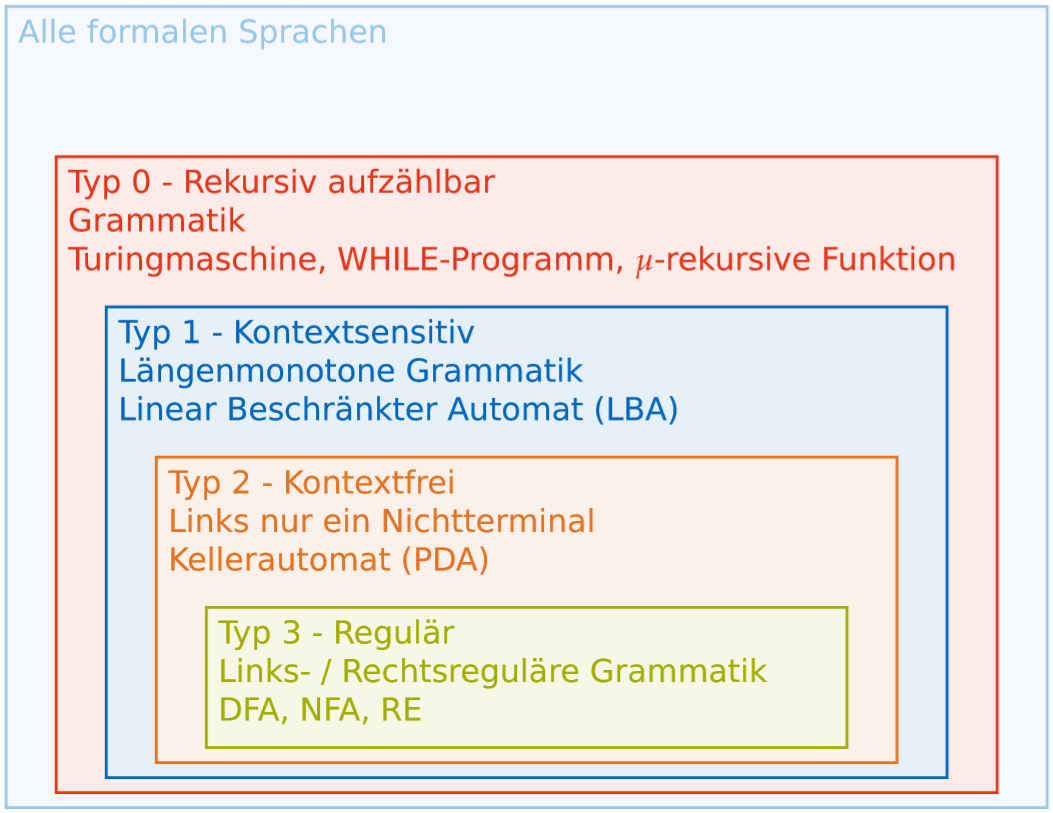
\includegraphics[width=0.75\textwidth]{../figures/Chomsky.png}
    \end{center}
\end{frame}

{\setbeamercolor{palette primary}{bg=ExColor}
\begin{frame}{Reguläre Grammatik}
    \begin{alertblock}{Aufgaben}
    Finde eine reguläre Grammatik für die folgenden Sprachen
    \end{alertblock}
    \metroset{block=fill}
    \begin{block}{Normal}
    \begin{itemize}
        \item $L_1 = \{a^{2n} \mid n\in\naturals\}$
        \item $L_2 = \{a^nb^m \mid n, m\in\naturals\}$
        \item $L_3 = \{uv \mid u\in\{a,b\}^\ast,\ v\in\{c,d\}\}$
        \item $L_4 = \{w \mid |w| = 3, w\in \{a,b,c\}^*\}$
    \end{itemize}
    \end{block}
    \begin{block}{Etwas Schwerer}
    \begin{itemize}
        \item $L_5 = \{a^n \mid n \equiv 1 \mod 3\}$
        \item $L_6 = \{uv\mid u\in\{\text{\Rewind, \MoveUp, \Forward, \MoveDown}\}^\ast,\;v\in\{\text{\Stopsign}\}\}$
        \item $L_7 = \{w \in \{a,b,c\}^* \mid |w|_a = 3, |w|_b = 1\}$
    \end{itemize}
    \end{block}
\end{frame}
}

{\setbeamercolor{palette primary}{bg=ExColor}
\begin{frame}{Lösung}
    \begin{itemize}
        \item<1-> \alert<1>{$P_1 = \{S \to aA \mid \emptyWord,\ A \to aB \mid a,\ B \to aA\}$}
        \item<2-> \alert<2>{$P_2 = \{S \to aA \mid bB \mid b \mid a \mid \emptyWord,\ A \to aA \mid bB \mid b \mid a ,\ B \to bB \mid b\}$}
        \item<3-> \alert<3>{$P_3 = \{S \to aS \mid bS \mid c \mid d\}$}
        \item<4-> \alert<4>{$P_4 = \{S \to aA \mid bA \mid cA,\ A \to aB \mid bB \mid cB,\ B \to a \mid b \mid c\}$}
        \item<5-> \alert<5>{$P_5 = \{S \to aA \mid a,\ A \to aB,\ B \to aS\}$}
        \item<6-> \alert<6>{$P_6 = \{S \to \text{\Rewind}S \mid \text{\MoveUp}S \mid \text{\Forward}S \mid \text{\MoveDown}S \mid \text{\Stopsign}\}$}
    \end{itemize}
\end{frame}
}

{\setbeamercolor{palette primary}{bg=ExColor}
\begin{frame}{Lösung}
        \begin{itemize}
            \item 
                \alert<1>{
                $P_7 = \{S \to cS \mid aA_1 \mid bB_0,$\\
                \vspace*{0.9mm}
                \hspace*{7mm}
                $\begin{aligned}
                A_1 &\to cA_1 \mid aA_2 \mid bB_1,\\
                A_2 &\to cA_2 \mid aA_3 \mid bB_2,\\
                A_3 &\to cA_3 \mid bB_3 \mid b,\\
                B_0 &\to cB_0 \mid aB_1,\\
                B_1 &\to cB_1 \mid aB_2,\\
                B_2 &\to cB_2 \mid aB_3 \mid a,\\
                B_3 &\to cB_3 \mid cC \mid c,\\
                C_{\;} &\to cC_{\;}\mid c\}
                \end{aligned}
                $}
        \end{itemize}
\end{frame}
}


\begin{frame}[standout]
  Murmelpause
\end{frame}

\section{Automaten}

\begin{frame}[fragile]{Reguläre Sprachen anders beschreiben}
    Wir können reguläre Sprachen auch graphisch beschreiben.\\
    Dafür nutzen wir \alert{endliche Automaten}.\\
    Ein Automat prüft Wörter und entscheidet, ob sie Teil der Sprache sind oder nicht.\\
    $\leadsto$ Wir nennen das \alert{\emph{akzeptieren}}, bzw. nicht akzeptieren.
    \begin{alertblock}{Funktionsweise}
        \begin{enumerate}
            \item Ein Wort wird in den Automat eingegeben
            \item Wort wird zeichenweise abgearbeitet
            \item Nach jedem Zeichen wird der Automat in einen Zustand überführt, der bestimmt, wie fortgefahren wird
            \item Befindet sich der Automat in einem \emph{Endzustand}, sobald das Wort abgearbeitet wurde, akzeptiert der Automat das Wort.
        \end{enumerate}
    \end{alertblock}
\end{frame}

\subsection{NEA}
\begin{frame}[fragile]{Bestandteile eines endlichen Automaten}
    Der Automat kann als gerichteter Graph notiert werden.\\
    Wir konstruieren ihn aus den folgenden Komponenten:
    \only<1|handout:1>{
        \begin{alertblock}{Startzustand}
            Im Startzustand wird das Wort eingegeben.\\
            \begin{center}
                \begin{tikzpicture}[->,>=stealth',shorten >=1pt,auto,node distance=2cm,semithick]
                    \node[initial,state](q0){$q_0$};
                \end{tikzpicture}
            \end{center}
        \end{alertblock}
    }
    \only<2|handout:1>{
        \begin{alertblock}{Zustandsübergang}
            Wird das Zeichen auf dem Übergang \emph{gelesen}, geht der Automat in den folgenden Zustand über.\\
            \begin{center}
                \begin{tikzpicture}[->,>=stealth',shorten >=1pt,auto,node distance=2cm,semithick]
                    \node[state](qi){$q_i$};
                    \node[state](qj)[right of=qi]{$q_j$};
                    \path (qi) edge node {$a$} (qj);
                \end{tikzpicture}
            \end{center}
        \end{alertblock}
    }
    \only<3|handout:2>{
        \begin{alertblock}{Endzustand}
            Falls sich der Automat in diesem Zustand befindet, und das Wort abgearbeitet ist, wird das Wort akzeptiert.\\
            \begin{center}
                \begin{tikzpicture}[->,>=stealth',shorten >=1pt,auto,node distance=2cm,semithick]
                    \node[accepting,state](qe){$q_E$};
                \end{tikzpicture}
            \end{center}
            \emph{Anmerkung: }Unter Umständen sind mehrere hiervon nötig
        \end{alertblock}
    }
\end{frame}

\begin{frame}[fragile]{Beispiel}
    \begin{exampleblock}{$L=\{axb \mid x\in\{a,b\}^\ast\}$}
        \vspace{0.3cm}
        \begin{tikzpicture}[->,>=stealth',shorten >=1pt,auto,node distance=2cm,
                semithick]
            %\tikzstyle{every state}=[fill=ExColor,draw=none,text=white]

            \node<1,3-> [initial,state]         (1)               {$q_0$};
            \node<2>    [initial,state,orange]  (1)               {$q_0$};
            \node       [state]                 (2) [right of=1]  {$q_1$};
            \node<1-8>  [state,accepting]       (3) [right of=2]  {$q_E$};
            \node<9>    [state,accepting,orange](3) [right of=2]  {$q_E$};

            \path<1,2,9>
            (1) edge                node {a}  (2)
            (2) edge [loop above]   node {a,b}(2)
            edge                node {b}  (3);
            \path<3>
            (1) edge [orange]       node {a}  (2)
            (2) edge [loop above]   node {a,b}(2)
            edge                node {b}  (3);
            \path<4,5,6,7>
            (1) edge                     node {a}  (2)
            (2) edge [loop above,orange] node {a,b}(2)
            edge                     node {b}  (3);
            \path<8>
            (1) edge                node {a}  (2)
            (2) edge [loop above]   node {a,b}(2)
            edge [orange]       node {b}  (3);
        \end{tikzpicture}
    \end{exampleblock}
    \onslide<2->{
        \begin{exampleblock}{Worteingabe:} \alert<3>{a}\alert<4>{a}\alert<5>{b}\alert<6>{a}\alert<7>{b}\alert<8>{b} $\in L$\only<1-8>{?} \only<9>{$\leadsto$ \alert{akzeptiert}
            }
        \end{exampleblock}}
\end{frame}

\begin{frame}{Beispiel: Automat}
    Gegeben ist eine Sprache L. Gesucht ist ein Automat M, der \textbf{genau} die Wörter aus L akzeptiert.
    \vspace{0.5cm}
    % \only<1>{
    % \begin{alertblock}{$L_1 = \{a^{2n} \mid n\in\naturals\}$}
    % \begin{tikzpicture}[->,>=stealth',shorten >=1pt,auto,node distance=2cm,semithick]
    %         \node   [initial,state,accepting]                   (1) {$q_0$};
    %         \node   [state]                     [right of=1]    (2) {$q_1$};
    %         \node   [state, accepting]          [right of=2]    (3) {$q_2$};

    %         \path
    %                 (1) edge node {a} (2);

    %         \path
    %                 (2) edge [bend left] node {a} (3);

    %         \path
    %                 (3) edge [bend left] node {a} (2);
    %     \end{tikzpicture}
    % \end{alertblock}
    % }
    \only<1>{
        \begin{alertblock}{$L_1 = \{uv \mid u\in\{a,b\}^\ast,\;v\in\{c,d\}\}$}
            \begin{tikzpicture}[->,>=stealth',shorten >=1pt,auto,node distance=2cm,semithick]
                \node   [initial,state]                             (1) {$q_0$};
                \node   [state,accepting]           [right of=1]    (2) {$q_1$};

                \path   (1) edge node {c,d} (2)
                (1) edge [loop above] node {a,b} (1);
            \end{tikzpicture}
        \end{alertblock}
    }

\end{frame}

{\setbeamercolor{palette primary}{bg=ExColor}
\begin{frame}{Denkpause}
    \begin{small}
        \begin{alertblock}{knifflige Aufgabe}
            Wir entwerfen einen Automat zur Aufzugskontrolle.
            Der Aufzug hat folgende Möglichkeiten:\\
            $\Sigma =\{$\begin{footnotesize}
                \framebox{EG$\nearrow$1.OG} , \framebox{EG$\nearrow$2.OG} , \framebox{1.OG$\searrow$EG} , \framebox{1.OG$\nearrow$2.OG} , \framebox{2.OG$\searrow$EG} , \\\qquad\quad\;\framebox{2.OG$\searrow$1.OG} , \framebox{OFF}
            \end{footnotesize}$\}$
            \begin{itemize}
                \item Der Aufzug startet vom Erdgeschoss und darf sich nur aus Stockwerken bewegen, in denen er sich befindet.
                \item Der Aufzug kann nur im Erdgeschoss ausgeschaltet werden. Er kann dann keine Bewegung durchführen.
                \item Der Aufzug muss ausgeschaltet werden.
            \end{itemize}
        \end{alertblock}
        % \begin{footnotesize}
        %     \framebox{EG$\nearrow$2.OG} \framebox{2.OG$\searrow$EG} \framebox{OFF} $\in L$\\
        %     \framebox{2.OG$\searrow$EG} \framebox{OFF} \framebox{EG$\nearrow$1.OG} $\notin L$\\
        % \end{footnotesize}
        \alert{Zeichne einen Automaten an, dessen akzeptierte Sprache genau die Menge der korrekten Abläufe ist.}
    \end{small}
\end{frame}

\begin{frame}<handout:0>{Lösung}
    \begin{center}
        \begin{tikzpicture}[->,>=stealth',shorten >=1pt,auto,node distance=3.2cm,semithick]
            \node [initial,state]   (0)              {$q_0$};
            \node [state]           (1) [above of=0] {$q_1$};
            \node [state]           (2) [above of=1] {$q_2$};
            \node [state,accepting] (E) [right of=0] {$q_E$};

            \path   (0) edge [bend left=10] node [rotate=90,above] {\footnotesize\framebox{EG$\nearrow$1.OG}} (1)
            edge [below]      node {\footnotesize\framebox{OFF}} (E)
            edge [bend left=70] node {\footnotesize\framebox{EG$\nearrow$2.OG}} (2)
            (1) edge [bend left=10] node [rotate=90,above] {\footnotesize\framebox{1.OG$\nearrow$2.OG}} (2)
            edge [bend left=10] node [rotate=90,below] {\footnotesize\framebox{1.OG$\searrow$EG}} (0)
            (2) edge [bend left=10] node [rotate=90,below] {\footnotesize\framebox{2.OG$\searrow$1.OG}}(1)
            edge [bend left=70] node {\footnotesize\framebox{2.OG$\searrow$EG}} (0);
        \end{tikzpicture}
    \end{center}
\end{frame}
}

{\setbeamercolor{palette primary}{bg=ExColor}
\begin{frame}{Denkpause}
    \begin{alertblock}{Aufgaben}
        Finde Automaten, die \textbf{genau} folgende Sprachen erkennen.
    \end{alertblock}
    \metroset{block=fill}
    \begin{block}{Normal}
        \begin{itemize}
            \item $L_1 = \{a^nb^m \mid n, m\in\naturals\}$
            \item $L_2 = \{w \mid |w| = 3, w\in \{a,b,c\}^*\}$
            \item $L_3 = \{uv \mid u\in\{\text{\Rewind, \MoveUp, \Forward, \MoveDown}\}^\ast,\;v\in\{\text{\Stopsign}\}\}$
        \end{itemize}
    \end{block}
    \begin{block}{Etwas Schwerer}
        \begin{itemize}
            \item $L_4 = \{a^n \mid n \equiv 1 \bmod 3\}$
            \item $L_5 = \{w \in \{a,b,c\}^* \mid |w|_a = 3, |w|_b = 1\}$
            \item $L_6=\{w \in \{a,b\}^* \mid |w|_a \equiv |w|_b \bmod 3\}$
        \end{itemize}
    \end{block}
\end{frame}
}



{\setbeamercolor{palette primary}{bg=ExColor}
\begin{frame}<handout:0>{Lösung}
    % \begin{itemize}[<+- | alert@+>]
    %     \item 
    \onslide<1->{\alert<1>{
        % \item
        \begin{tikzpicture}[->,>=stealth',shorten >=1pt,auto,node distance=2cm,semithick]
            \node   [initial,state,accepting]                   (1) {$q_0$};
            \node   [state,accepting]           [right of=1]    (2) {$q_1$};

            \path   (1) edge node {b} (2)
            (1) edge [loop above] node {a} (1);

            \path   (2) edge [loop above] node {b} (2);
        \end{tikzpicture}
    }}
    \vspace{0.2cm}
    \onslide<2->{\alert<2>{
        \begin{tikzpicture}[->,>=stealth',shorten >=1pt,auto,node distance=2cm,semithick]
            \node   [initial,state]                             (1) {$q_0$};
            \node   [state]             [right of=1]            (2) {$q_1$};
            \node   [state]             [right of=2]            (3) {$q_2$};
            \node   [state,accepting]   [right of=3]            (4) {$q_3$};

            \path   (1) edge node {a,b,c} (2);
            \path   (2) edge node {a,b,c} (3);
            \path   (3) edge node {a,b,c} (4);
        \end{tikzpicture}
    }}
    \vspace{0.2cm}
    \onslide<3->{\alert<3>{
        \begin{tikzpicture}[->,>=stealth',shorten >=1pt,auto,node distance=2cm,semithick]
            \node   [initial,state]         (1) {$q_0$};
            \node   [state,accepting]   [right of=1]       (2) {$q_1$};

            \path   (1) edge    [loop above]    node    {\text{\Rewind, \MoveUp, \Forward, \MoveDown}} (1)
            (1) edge                    node    {$\text{\Stopsign}$}   (2);
        \end{tikzpicture}}}
    \vspace{0.2cm}
    \onslide<4->{\alert<4>{
        \begin{tikzpicture}[->,>=stealth',shorten >=1pt,auto,node distance=2cm,semithick]
            \node   [initial,state]                             (1) {$q_0$};
            \node   [state,accepting]   [right of=1]            (2) {$q_1$};
            \node   [state]             [right of=2]            (3) {$q_2$};

            \path   (1) edge node {a} (2);
            \path   (2) edge node {a} (3);
            \path   (3) edge [bend left] node {a} (1);
        \end{tikzpicture}
    }}
    % \end{itemize}
\end{frame}
}

{\setbeamercolor{palette primary}{bg=ExColor}
\begin{frame}<handout:0>{Lösung}
    \onslide<1->{\alert<1>{
        \begin{tikzpicture}[->,>=stealth',shorten >=1pt,auto,node distance=1.5cm,semithick]
            \node   [initial,state]                             (1) {$q_0$};
            \node   [state]             [right of=1]            (2) {$q_1$};
            \node   [state]             [right of=2]            (3) {$q_2$};
            \node   [state]             [right of=3]            (4) {$q_3$};
            \node   [state]             [below of=1]             (5) {$q_4$};
            \node   [state]             [below of=2]             (6) {$q_5$};
            \node   [state]             [below of=3]             (7) {$q_6$};
            \node   [state, accepting]  [below of=4]             (8) {$q_7$};

            \path   (1) edge node {a} (2)
            (1) edge node {b} (5)
            (1) edge [loop above] node {c} (1);

            \path   (2) edge node {a} (3)
            (2) edge node {b} (6)
            (2) edge [loop above] node {c} (2);

            \path   (3) edge node {a} (4)
            (3) edge node {b} (7)
            (3) edge [loop above] node {c} (3);

            \path   (4) edge node {b} (8)
            (4) edge [loop above] node {c} (4);

            \path   (5) edge node {a} (6)
            (5) edge [loop below] node {c} (5);

            \path   (6) edge node {a} (7)
            (6) edge [loop below] node {c} (6);

            \path   (7) edge node {a} (8)
            (7) edge [loop below] node {c} (7);

            \path   (8) edge [loop below] node {c} (8);
        \end{tikzpicture}
    }}
\end{frame}
}

{\setbeamercolor{palette primary}{bg=ExColor}
\begin{frame}<handout:0>{Lösung}
    \onslide<1->{\alert<1>{
        \begin{tikzpicture}[->,>=stealth',shorten >=1pt,auto,node distance=4cm,semithick]
            \node   [initial,state,accepting]                             (1) {$q_0$};
            \node   [state]             [right of=1]            (2) {$q_1$};
            \node   [state]             [below of=1]            (3) {$q_2$};

            \path   (1) edge [bend right] node {a} (2)
            (1) edge [bend right] node {b} (3);
            \path   (2) edge node {a} (3)
            (2) edge [bend right] node {b} (1);
            \path   (3) edge [bend right] node {a} (1)
            (3) edge [bend right=60] node {b} (2);
        \end{tikzpicture}
    }}
\end{frame}
}


\begin{frame}[standout]
  Murmelpause
\end{frame}

% Copyright 2018, 2019, 2020, 2021 FIUS
%
% This file is part of theo-vorkurs-folien.
%
% theo-vorkurs-folien is free software: you can redistribute it and/or modify
% it under the terms of the GNU General Public License as published by
% the Free Software Foundation, either version 3 of the License, or
% (at your option) any later version.
%
% theo-vorkurs-folien is distributed in the hope that it will be useful,
% but WITHOUT ANY WARRANTY; without even the implied warranty of
% MERCHANTABILITY or FITNESS FOR A PARTICULAR PURPOSE.  See the
% GNU General Public License for more details.
%
% You should have received a copy of the GNU General Public License
% along with theo-vorkurs-folien.  If not, see <https://www.gnu.org/licenses/>.

\subsection{DEA}
\begin{frame}[fragile]{Deterministische endliche Automaten}
    \begin{alertblock}{Wir beschränken unseren Automaten folgendermaßen:}
        Von \alert{jedem Zustand} muss \alert{genau ein} Übergang für \alert{jedes $a\in\Sigma$} ausgehen.
    \end{alertblock}
    %\vspace{0.3}
    \onslide<2->{
        Um dies zu ermöglichen führen wir eine neue Komponente ein:
        \begin{alertblock}{Fangzustand}
            Dieser Zustand kann nicht verlassen werden.\\
            Falls der Automat in diesem Zustand landet, kommt er nicht mehr raus. Das Wort kann nicht akzeptiert werden.
            \begin{center}
                \begin{tikzpicture}[->,>=stealth',shorten >=1pt,auto,node distance=2cm,semithick]
                    \node[state](qi){$q_f$};
                    \path (qi) edge [loop right] node {$x \in \Sigma$} (B);
                \end{tikzpicture}
            \end{center}
        \end{alertblock}
    }
\end{frame}

\begin{frame}[fragile]{Beispiel}
    \begin{exampleblock}{$L=\{axb \mid x\in\{a,b\}^\ast\}$}
        \vspace{0.3cm}
        \begin{tikzpicture}[->,>=stealth,shorten >=1pt,auto,node distance=2cm,
                semithick]
            %\tikzstyle{every state}=[fill=ExColor,draw=none,text=white]

            \node<1,3-> [initial,state]         (1)               {$q_0$};
            \node<2>    [initial,state,orange]  (1)               {$q_0$};
            \node       [state]                 (2) [right of=1]  {$q_1$};
            \node<1-8>  [state,accepting]       (3) [right of=2]  {$q_E$};
            \node<9>    [state,accepting,orange](3) [right of=2]  {$q_E$};
            \node       [state]                 (4) [below of=1]  {$q_f$};

            \path<1,2,9>
            (1) edge                node {$a$}  (2)
            edge                node {$b$}  (4)
            (2) edge [loop above]   node {$a$}  (2)
            edge [bend left]    node {$b$}  (3)
            (4) edge [loop right]   node {$a,b$}(4)
            (3) edge [loop above]   node {$b$}  (3)
            edge [bend left]    node {$a$}  (2);
            \path<3>
            (1) edge [orange]       node {$a$}  (2)
            edge                node {$b$}  (4)
            (2) edge [loop above]   node {$a$}  (2)
            edge [bend left]    node {$b$}  (3)
            (4) edge [loop right]   node {$a,b$}(4)
            (3) edge [loop above]   node {$b$}  (3)
            edge [bend left]    node {$a$}  (2);
            \path<4>
            (1) edge                node {$a$}  (2)
            edge                node {$b$}  (4)
            (2) edge [loop above,orange] node {$a$}  (2)
            edge [bend left]    node {$b$}  (3)
            (4) edge [loop right]   node {$a,b$}(4)
            (3) edge [loop above]   node {$b$}  (3)
            edge [bend left]    node {$a$}  (2);
            \path<5,7>
            (1) edge                node {$a$}  (2)
            edge                node {$b$}  (4)
            (2) edge [loop above]   node {$a$}  (2)
            edge [bend left,orange] node {$b$}  (3)
            (4) edge [loop right]   node {$a,b$}(4)
            (3) edge [loop above]   node {$b$}  (3)
            edge [bend left]    node {$a$}  (2);
            \path<6>
            (1) edge                node {$a$}  (2)
            edge                node {$b$}  (4)
            (2) edge [loop above]   node {$a$}  (2)
            edge [bend left]    node {$b$}  (3)
            (4) edge [loop right]   node {$a,b$}(4)
            (3) edge [loop above]   node {$b$}  (3)
            edge [bend left,orange] node {$a$}  (2);
            \path<8>
            (1) edge                node {$a$}  (2)
            edge                node {$b$}  (4)
            (2) edge [loop above]   node {$a$}  (2)
            edge [bend left]    node {$b$}  (3)
            (4) edge [loop right]   node {$a,b$}(4)
            (3) edge [loop above,orange] node {$b$}  (3)
            edge [bend left]    node {$a$}  (2);
        \end{tikzpicture}
    \end{exampleblock}
    \onslide<2->{
        \begin{exampleblock}{Worteingabe:} \alert<3>{$a$}\alert<4>{$a$}\alert<5>{$b$}\alert<6>{$a$}\alert<7>{$b$}\alert<8>{$b$} $\in L$\only<1-8>{?} \only<9>{$\leadsto$ \alert{akzeptiert}
            }
        \end{exampleblock}}
\end{frame}

{\setbeamercolor{palette primary}{bg=ExColor}
\begin{frame}{Denkpause}
    \footnotesize
    \begin{alertblock}{Aufgaben}
        Finde deterministische endliche Automaten (DEAs) für die folgenden Sprachen.
    \end{alertblock}
    \metroset{block=fill}
    \begin{block}{Normal}
        \begin{itemize}
            \item $L_1 = \{a^{2n} \mid n \in \mathbb{N}\}$ über $\Sigma=\{a\}$
            \item $L_2 = \{w\in \{a,b\}^* \mid |w|_a \geq 2\}$ über $\Sigma=\{a,b\}$
        \end{itemize}
    \end{block}
    \begin{block}{Prüfungsaufgabe: Etwas Schwerer}
        \begin{itemize}
            \item $L_3 = \{w \in \{a, b, c\}^* \mid \; |w|_b \geq 1$ und $aaca$ ist Suffix von w$\}$ über $\Sigma=\{a,b,c\}$
        \end{itemize}
    \end{block}
    \begin{block}{Prüfungsaufgabe: Schwer}
        \begin{itemize}
            \item $L_4 = \{bin(n)\mid \exists k \in \mathbb{N}: n=4k, bin(n)\text{ ist Binärdarstellung von }n\}$ über $\Sigma=\{1,0\}$\\
                  \emph{Achtung: Keine führenden Nullen.}
        \end{itemize}
    \end{block}
\end{frame}
}

{\setbeamercolor{palette primary}{bg=ExColor}
\begin{frame}<handout:0>{Lösung: Normal}
    \only<1->{
        \begin{alertblock}{$L_1 = \{a^{2n} \mid n \in \mathbb{N}\}$}
            \begin{tikzpicture}[->,>=stealth',shorten >=1pt,auto,node distance=2cm,
                    semithick]
                \node [initial,state,accepting] (0)              {$q_0$};
                \node [state]                   (1) [right of=0] {$q_1$};
                \path   (0) edge [bend left]   node {$a$} (1)
                (1) edge [bend left]   node {$a$} (0);
            \end{tikzpicture}
        \end{alertblock}}

    \only<2->{
        \begin{alertblock}{$L_2 = \{w\in \{a,b\}^* \mid |w|_a \geq 2\}$}
            \begin{tikzpicture}[->,>=stealth',shorten >=1pt,auto,node distance=2cm,
                    semithick]
                \node [initial,state]   (0)              {$q_0$};
                \node [state]           (1) [right of=0] {$q_1$};
                \node [state,accepting] (2) [right of=1] {$q_2$};
                \path   (0) edge               node {$a$} (1)
                edge [loop above]  node {$b$} (1)
                (1) edge               node {$a$} (2)
                edge [loop above]  node {$b$} (2)
                (2) edge [loop above]  node {$a,b$}(2);
            \end{tikzpicture}
        \end{alertblock}}
\end{frame}
}

{\setbeamercolor{palette primary}{bg=ExColor}
\begin{frame}<handout:0>{Lösung: Prüfungsaufgabe: Etwas Schwerer}
    \begin{alertblock}{$L_3 = \{w \in \{a, b, c\}^* \mid \; |w|_b \geq 1$ und $aaca$ ist Suffix von w$\}$}
        \begin{tikzpicture}[->,>=stealth',shorten >=1pt,auto,node distance=1.5cm,
                semithick]
            \node [initial,state]   (0)              {$q_0$};
            \node [state]           (1) [right of=0] {$q_1$};
            \node [state]           (2) [right of=1] {$q_2$};
            \node [state]           (3) [right of=2] {$q_3$};
            \node [state]           (4) [right of=3] {$q_4$};
            \node [state,accepting] (5) [right of=4] {$q_E$};

            \path
            (0) edge                    node {$b$}    (1)
            edge [loop below]       node {$a,c$}  (0)
            (1) edge                    node {$a$}    (2)
            edge [loop below]       node {$b,c$}  (1)
            (2) edge                    node {$a$}    (3)
            edge [bend right=85]    node {$b,c$}  (1)
            (3) edge                    node {$c$}    (4)
            edge [bend left]        node {$b$}    (1)
            edge [loop below]       node {$a$}    (3)
            (4) edge                    node {$a$}    (5)
            edge [bend right=95]    node {$b,c$}  (1)
            (5) edge [bend left=60]     node {$b,c$}  (1)
            edge [bend left]        node {$a$}    (3);
        \end{tikzpicture}
    \end{alertblock}
\end{frame}

\begin{frame}<handout:0>{Lösung: Prüfungsaufgabe: Schwer}
    \begin{alertblock}{$L_4 = \{bin(n)\mid \exists k \in \mathbb{N}: n=4k, bin(n)\text{ ist Binärdarstellung von }n\}$}
        \begin{tikzpicture}[->,>=stealth',shorten >=1pt,auto,node distance=2cm,
                semithick]
            \node [initial,state]   (0)              {$q_0$};
            \node [state]           (1) [right of=0] {$q_1$};
            \node [state]           (2) [right of=1] {$q_2$};
            \node [state,accepting] (3) [below of=2] {$q_3$};
            \node [state,accepting] (4) [below of=0] {$q_4$};
            \node [state]           (5) [below of=1] {$q_f$};
            \path   (0) edge               node {1} (1)
            edge               node {0} (4)
            (1) edge               node {0} (2)
            edge [loop above]  node {1} (1)
            (2) edge               node {0} (3)
            edge [bend left]  node {1} (1)
            (3) edge [loop right]  node {0} (3)
            edge               node {1} (1)
            (4) edge               node {0,1}(5)
            (5) edge [loop below]  node {0,1}(5);
        \end{tikzpicture}
    \end{alertblock}
\end{frame}
}

% {\setbeamercolor{palette primary}{bg=ExColor}
% \begin{frame}{Denkpause}
%  \begin{alertblock}{Aufgaben}
%  Finde einen deterministischen Automaten für die folgenden Sprachen:
%  \end{alertblock}
%  \metroset{block=fill}
%  \begin{block}{Normal}
%  \begin{itemize}
%      \item $L_1 = \{a^{2n} \mid n\in\naturals\}$
%      \item $L_2 = \{a^nb^m \mid n, m\in\naturals\}$
%      \item $L_3 = \{uv \mid u\in\{a,b\}^\ast,\;v\in\{c,d\}\}$
%      \item $L_4 = \{w \mid |w| = 3, w\in \{a,b,c\}^*\}$
%  \end{itemize}
%  \end{block}
%  \begin{block}{Etwas Schwerer}
%  \begin{itemize}
%      \item $L_4 = \{a^n \mid n \equiv 1 \pmod 3\}$
%      \item $L_5 = \{w \mid |w|_a = 3, |w|_b = 1, w\in \{a,b,c\}^*\}$
%      \item $L_6 = \{uv \mid u\in\{\text{\Rewind, \MoveUp, \Forward, \MoveDown}\}^\ast,\;v\in\{\text{\Stopsign}\}\}$
%      \item
%  \end{itemize}
%  \end{block}
% \end{frame}
% }

% {\setbeamercolor{palette primary}{bg=ExColor}
% \begin{frame}{Lösungen}
% Alle Lösungen sind Beispiellösungen, es sind auch andere möglich.
%  \begin{itemize}[<+- | alert@+>]
%      \item bla
%  \end{itemize}
% \end{frame}
% }  



%ToDo
% - gute Aufgaben zu Automaten finden, die Spaß machen zu bearbeiten und interesse an theo fördern
%    - zB richtige Klammerung, Aufzug etc.
%    - grammatik labyrinth aufgabe nochmal, nur mit automaten
% - erst nea, dann dea, minimal nicht erwähnen
% - NEA vs DEA?
% - typ 3 grammatik kann das selbe wie endlicher automat
% - je nach zeit noch reguläre ausdrücke
% - möglichst so konstruieren, dass man an einige punkte hat an denen man bedenkenlos aus Zeitgründen aufhören kann


\begin{frame}[standout]
  Murmelpause
\end{frame}

\section{Grammatik und Automaten}

% Copyright 2018-2022 FIUS
%
% This file is part of theo-vorkurs-folien.
%
% theo-vorkurs-folien is free software: you can redistribute it and/or modify
% it under the terms of the GNU General Public License as published by
% the Free Software Foundation, either version 3 of the License, or
% (at your option) any later version.
%
% theo-vorkurs-folien is distributed in the hope that it will be useful,
% but WITHOUT ANY WARRANTY; without even the implied warranty of
% MERCHANTABILITY or FITNESS FOR A PARTICULAR PURPOSE.  See the
% GNU General Public License for more details.
%
% You should have received a copy of the GNU General Public License
% along with theo-vorkurs-folien.  If not, see <https://www.gnu.org/licenses/>.

\begin{frame}{Automaten und Grammatiken}
  \metroset{block=fill}
  \begin{exampleblock}{Satz}
    Jede durch \only<6-|handout:0>{\alert<6>{deterministische}} endliche Automaten erkennbare Sprache ist auch regulär (also Typ 3).
  \end{exampleblock}
  \onslide<2-|handout:1> %
  Sei \alert<2|handout:0>{$A \subseteq \SigmaStern$} eine Sprache und \alert<2|handout:0>{M ein \only<-5|handout:0>{Automat}\only<6-|handout:1>{\alert<6|handout:0>{DEA}}} mit \alert<2-3|handout:0>{$\mathbf{T(M) = A}$}.\\
  \onslide<3-|handout:1> %
  (d.h. $M$ erkennt die Sprache $A$) \\
  \vspace{.3cm} %

  \onslide<4-|handout:1> %
  Wir suchen eine \alert<4|handout:0>{Typ 3-Grammatik G} mit \alert<4-5|handout:0>{$\mathbf{L(G) = A}$}.\\
  \onslide<5-|handout:1> %
  (d.h. die Grammatik $G$ erzeugt die Sprache $A$)
  \vspace{.3cm} %

  \onslide<6-|handout:1> %
  \begin{alertblock}{Anmerkung}
    Wir beschränken uns auf DEAs; in der Vorlesung werdet ihr aber eine allgemeinere Äquivalenz zeigen.
  \end{alertblock}
\end{frame}

\begin{frame}{DEA zu Grammatik: Konstruktion}
  Also: \alert<4-5|handout:0>{Zustände $\hat{=}$ Variablen}; \alert<6|handout:0>{Übergänge $\hat{=}$ Produktionen}

  \onslide<2-|handout:1> %
  Sei also ein \alert<2|handout:0>{DEA $M = (\alert<4|handout:0>{Z}, \alert<3|handout:0>{\Sigma}, \alert<6|handout:0>{\delta}, \alert<5|handout:0>{z_0}, E)$} gegeben. \\
    Wir definieren die \alert<2|handout:0>{Grammatik $G = (\alert<4|handout:0>{V}, \alert<3|handout:0>{\Sigma}, \alert<6|handout:0>{P}, \alert<5|handout:0>{S})$} mit:
  \begin{itemize}
    \item<3- | alert@3|handout:1> Alphabet $\Sigma$
    \item<4- | alert@4|handout:1> Variablenmenge $V = Z$
    \item<5- | alert@5|handout:1> Startsymbol $S = z_0$
    \item<6- | alert@6|handout:1> Produktionsmenge $P$ erzeugen wir aus $\delta$
  \end{itemize}
\end{frame}

\begin{frame}{DEA zu Grammatik: Produktionsregeln}\begin{columns}
    \begin{column}{0.5\textwidth}
      Für die Produktionsmenge $P$ wandeln wir die Übergänge um. \\
      \vspace{.3cm}
      \onslide<2-|handout:1> %
      Jedem $\delta$-Übergang \alert<2-3|handout:0>{$\delta(z_1, a)=z_2$} ordnen wir folgende Regeln zu:
      \begin{itemize}
        \item<2- | alert@2|handout:1> $z_1 \rightarrow a z_2$
        \item<3-|handout:1> Und zusätzlich, falls \alert<3|handout:0>{$z_2 \in E:$ $z_1 \rightarrow a$}
      \end{itemize}
      \onslide<4-|handout:1>{ %
        Falls $z_0 \in E$, brauchen wir außerdem $z_0 \to \emptyWord$.
      }
    \end{column}
    \begin{column}{0.5\textwidth}\centering\alert<handout:0>{\only<2-3|handout:1>{ %
        \begin{tikzpicture}[->,>=stealth',shorten >=1pt,auto,node distance=2cm,semithick]
          \node [state] (1)  {$z_1$};
          \onslide<2|handout:1>{
            \node [state] (2) [right of=1]  {$z_2$};
            \path (1) edge node {a} (2);
          }\onslide<3|handout:1>{
            \node [state, accepting] (2') [right of=1]  {$z_2$};
            \path (1) edge node {a} (2');
          }
        \end{tikzpicture} \\
        \glqq$\delta (z_1,a) = z_2$\grqq \\
        wird zu
        \begin{align*}
           & z_1 \to az_2            \\
           & \onslide<3->{z_1 \to a}
        \end{align*}
      }\only<4|handout:1>{
        \begin{tikzpicture}[->,>=stealth',shorten >=1pt,auto,node distance=2cm,semithick]
          \node [state,initial,accepting] (0)  {$z_0$};
        \end{tikzpicture} \\
        \glqq$z_0 \in E$\grqq \\
        wird zu $$z_0 \to \emptyWord$$
      }}\end{column}
  \end{columns}\end{frame}

\begin{frame}{DEA zu Grammatik: Korrektheit (Beweisidee)}
  \begin{alertblock}{Zu zeigen: $x \in T(M)$ gdw. $x \in L(G)$}
    \onslide<2-|handout:1> %
    Sei $x = a_1 a_2 \ldots a_{n-1} a_n$ ein Wort, das von $M$ akzeptiert wird. \\
    \onslide<3-|handout:1> %
    \begin{center}\centering\begin{tikzpicture}[->,>=stealth',shorten >=1pt,auto,node distance=1.75cm,semithick]
        \alert<5-5|handout:0>{\node [initial,state]   (0)              {$z_0$};}
        \alert<5-6|handout:0>{\node [state]           (1) [right of=0] {$z_1$};}
        \alert<6-8|handout:0>{\node                   (5) [right of=1] {$\ldots$};}
        \alert<8-9|handout:0>{\node [state]           (8) [right of=5] {$z_{n-1}$};}
        \alert<9-9|handout:0>{\node [state,accepting] (9) [right of=8] {$z_n$};}

        \alert<5|handout:0>{\path (0) edge node {$a_1$}     (1);}
        \alert<6|handout:0>{\path (1) edge node {$a_2$}     (5);}
        \alert<8|handout:0>{\path (5) edge node {$a_{n-1}$} (8);}
        \alert<9|handout:0>{\path (8) edge node {$a_n$}     (9);}
      \end{tikzpicture}\end{center}
    \onslide<4-|handout:1> %
    Mit den passenden Regeln \only<5-9|handout:1>{(z.B. %
      \only<5>{$z_0 \to a_1 z_1$}%
      \only<6>{$z_1 \to a_2 z_2$}%
      \only<7>{$z_2 \to a_3 z_3$}%
      \only<8>{$z_{n-2} \to a_{n-1} z_{n-1}$}%
      \only<9>{$z_{n-1} \to a_n$}%
      ) }lässt sich $x$ ableiten:
    $$\alert<5|handout:0>{z_0} \alert<5|handout:0>{\Rightarrow} \alert<5|handout:0>{a_1} \alert<5-6|handout:0>{z_1} \alert<6|handout:0>{\Rightarrow} a_1 \alert<6|handout:0>{a_2} \alert<6-7|handout:0>{z_2} \alert<7|handout:0>{\Rightarrow} \alert<7-8|handout:0>{\ldots} \alert<8|handout:0>{\Rightarrow} a_1 a_2 \ldots \alert<8|handout:0>{a_{n-1}} \alert<8-9|handout:0>{z_{n-1}} \alert<9|handout:0>{\Rightarrow} a_1 a_2 \ldots a_{n-1} \alert<9|handout:0>{a_n} = x$$
    \onslide<10-|handout:1> %
    Also können wir das Wort in der Grammatik ableiten. \\
    \onslide<11-|handout:1> %
    \alert<11|handout:0>{Funktioniert die Argumentation auch andersrum?}
    \onslide<12-|handout:1> %
    \alert<12|handout:0>{Ja!}
  \end{alertblock}
\end{frame}

\begin{frame}{DEA zu Grammatik: Korrektheit}
  \begin{alertblock}{Zu zeigen: $x \in T(M)$ gdw. $x \in L(G)$}
    Dabei gilt immer noch: $x = a_1 a_2 \ldots a_{n-1} a_n$ \\
    \onslide<2-|handout:1> %
    Die folgenden Aussagen sind äquivalent:
    \begin{itemize}
      \item<3- | alert@3|handout:1|handout:alert@0> $x$ wird von Automat $M$ erkannt \emph{$(x\in T(M))$}
      \item<4- | alert@4|handout:1|handout:alert@0> Es gibt eine Folge von Zuständen $z_0, z_1, \ldots, z_{n-1}, z_n$ mit:
            $z_0$ ist Startzustand, $z_n$ ist Endzustand \textbf{und}:
            $\forall i \in \{1, \ldots, n\}: \delta(z_{i-1}, a_i) = z_i$
      \item<5- | alert@5|handout:1|handout:alert@0> Es gibt Folge an Variablen $z_0, z_1, \dots, z_{n-1}$ mit:
            $z_0$ ist Startvariable, $(z_{n-1} \to a_n) \in P$ \textbf{und}:
            $\forall i \in \{1, \ldots, n-1\}: (z_{i-1} \to a_i z_i) \in P$
      \item<6- | alert@6|handout:1|handout:alert@0> Es gibt Folge an Variablen $z_0, z_1, \dots, z_{n-1}$ mit:
            $z_0$ ist Startvariable \textbf{und}: $z_0 \Rightarrow a_1 z_1 \Rightarrow \ldots \Rightarrow a_1 a_2 \ldots a_{n-1} a_n$
      \item<7- | alert@7|handout:1|handout:alert@0> x wird von der Grammatik G produziert \emph{$(x \in L(G))$}
    \end{itemize}
    \onslide<8-|handout:1> %
    Also gilt die Äquivalenz. \qed
  \end{alertblock}
\end{frame}

% \begin{frame}[fragile]{Grammatik zu Automaten}
%  Eine reguläre Grammatik und eine endlicher Automat können die selben Sprachen beschreiben.
%  \begin{exampleblock}{\glqq$\implies$\grqq}
%  \only<1>{Aus $z_1 \to az_2 \in P$ wird:\\
%  \begin{center}
%  \vspace{0.3cm}
%      \begin{tikzpicture}[->,>=stealth',shorten >=1pt,auto,node distance=2cm,
%                      semithick]
%      %\tikzstyle{every state}=[fill=ExColor,draw=none,text=white]

%      \node       [state]                 (1) [right of=1]  {$z_1$};
%      \node       [state]                 (2) [right of=2]  {$z_2$};

%      \path
%              (1) edge                node {a}  (2);
%      \end{tikzpicture}\\
%      \glqq$\delta (z_1,a) = z_2$\grqq
%  \end{center}}

%  \only<2>{
%  Falls $z_2 \in F$ ($z_2$ ein Endzustand)\\
%  Aus $z_1 \to a \in P$ wird:\\
%  \begin{center}
%  \vspace{0.3cm}
%      \begin{tikzpicture}[->,>=stealth',shorten >=1pt,auto,node distance=2cm,
%                      semithick]
%      %\tikzstyle{every state}=[fill=ExColor,draw=none,text=white]

%      \node       [state]                 (1) [right of=1]  {$z_1$};
%      \node       [state, accepting]      (2) [right of=2]  {$z_2$};

%      \path
%              (1) edge                node {a}  (2);
%      \end{tikzpicture}\\
%      \glqq$\delta (z_1,a) = z_2$\grqq
%  \end{center}
%  }
%  \end{exampleblock}
% \end{frame}


\begin{frame}[standout]
  Murmelpause
\end{frame}

\section{Reguläre Ausdrücke}

\begin{frame}[fragile]{mehr Möglichkeiten reguläre Sprachen zu beschreiben}
    Graphen und \glqq Bilder\grqq\ sind oft nicht das optimale Mittel eine Sprache zu beschreiben.\\
    Die \alert{regulären Ausdrücke} bieten uns eine Möglichkeit Sprachen schnell und intuitiv zu beschreiben.
    \begin{alertblock}{Funktionsweise}
        \begin{enumerate}
            \item Wörter können mit einem angegebenen Muster abgeglichen werden.
            \item Lässt sich ein Wort durch das Muster beschreiben, ist es in der davon beschriebenen Sprache.
        \end{enumerate}
    \end{alertblock}
\end{frame}

\begin{frame}{Reguläre Ausdrücke verwenden}
    \begin{alertblock}{Induktive Definition der Syntax}
        \begin{itemize}
            \item \alert{$\emptyset$} und \alert{$\emptyWord$} sind reguläre Ausdrücke.
            \item \alert{a} ist ein regulärer Ausdruck (für alle a $\in \Sigma$).
            \item Wenn \alert{$\alpha$} und \alert{$\beta$} reguläre Ausdrücke sind,\\dann sind \alert{$\alpha \beta$}, \alert{($\alpha \mid \beta$)} und \alert{$(\alpha)^*$} auch reguläre Ausdrücke.
        \end{itemize}
    \end{alertblock}
    \metroset{block=fill}
    \begin{exampleblock}{Beispiel}
        $\gamma = ((a|b)^* \mid \emptyWord) \implies aba \in L(\gamma)$
    \end{exampleblock}
\end{frame}

\begin{frame}{Reguläre Ausdrücke verwenden}
    \begin{exampleblock}{Wie Sprachen und reguläre Ausdrücke zusammenhängen}
        \footnotesize
        \begin{itemize}[<+- | alert@+>]
            \item Wenn $\gamma = \emptyset$, beschreibt es die leere Sprache: $L(\gamma) = \{\}$
            \item Wenn $\gamma$ ein einzelnes Wort ist, ist genau dieses Wort in der Sprache enthalten.\\
                  $\gamma = \emptyWord$: $L(\gamma)=\{\emptyWord\}$,\quad$\gamma = a$: $L(\gamma)=\{a\}$
            \item Wenn $\gamma$ aus zwei hintereinandergeschrieben Ausdrücken besteht, repräsentiert Konkatenation.\\
                  $\gamma = (a)^*b: L(\gamma)=\{a^nb \mid n \in \mathbb{N}\}$
            \item Wenn $\gamma$ aus zwei mit \glqq oder\grqq\ verknüpften Ausdrücken besteht, sind beide Seiten in der Sprache enthalten.\\
                  $\gamma = (a \mid bc)$: $L(\gamma)=\{a, bc\}$
            \item Wenn $\gamma$ ein Ausdruck mit einem Stern ist, kann dieser innere Ausdruck beliebig oft wiederholt werden (auch null mal).\\
                  $\gamma = (a)^*$: $L(\gamma)=\{\emptyWord, a, aa, aaa, ...\}=\{a\}^*$
            \item Alles zusammen --- $\gamma = ((a)^* \mid (bc)^*)$: $L(\gamma)=\{\emptyWord, a, bc, aa, bcbc, aaa, ...\} = \{a\}^* \cup \{bc\}^*$
        \end{itemize}
    \end{exampleblock}
\end{frame}

{\setbeamercolor{palette primary}{bg=ExColor}
\begin{frame}{Reguläre Ausdrücke}
    \begin{alertblock}{Aufgaben}
        Finde einen regulären Ausdruck für die folgenden Sprachen
    \end{alertblock}
    \metroset{block=fill}
    \begin{block}{Normal}
        \begin{itemize}
            \item $L(\gamma_1) = \{a^{2n} \mid n\in\naturals\}$
            \item $L(\gamma_2) = \{a^nb^m \mid n, m\in\naturals\}$
            \item $L(\gamma_3) = \{uv \mid u\in\{a,b\}^\ast,\ v\in\{c,d\}\}$
            \item $L(\gamma_4) = \{w \mid |w| = 3, w\in \{a,b,c\}^*\}$
        \end{itemize}
    \end{block}
    \begin{block}{Etwas Schwerer}
        \begin{itemize}
            \item $L(\gamma_5) = \{a^n \mid n \equiv 1 \mod 3\}$
            \item $L(\gamma_6) = \{uv\mid u\in\{\text{\Rewind, \MoveUp, \Forward, \MoveDown}\}^\ast,\;v\in\{\text{\Stopsign}\}\}$
            \item $L(\gamma_7) = \{w \mid |w|_a = 3, |w|_b = 1, w\in \{a,b,c\}^*\}$
        \end{itemize}
    \end{block}
\end{frame}
}

{\setbeamercolor{palette primary}{bg=ExColor}
\begin{frame}<handout:0>{Lösung}
    Alle Lösungen sind Beispiellösungen, es sind auch andere möglich.\\
    Klammern die nicht zur Bedeutung beitragen, dürfen wir für die Kurzschreibweise weglassen.
    \begin{itemize}[<+- | alert@+>]
        \item $\gamma_1 = (aa)^*$
        \item $\gamma_2 = (a)^*(b)^*$
        \item $\gamma_3 = (a|b)^*\ (c|d)$
        \item formal: $\gamma_4 = ((a|b)|c)((a|b)|c)((a|b)|c)$, kurz: $\gamma_4 = (a|b|c)(a|b|c)(a|b|c)$
        \item $\gamma_5 = a(aaa)^*$
        \item formal: $\gamma_6 = ($((\Rewind | \MoveUp) | \Forward) | \MoveDown$)^*$\Stopsign, kurz: $\gamma_6 = ($\Rewind | \MoveUp | \Forward | \MoveDown$)^*$\Stopsign
        \item formal: $\gamma_7 = (c)^*(a(c)^*a(c)^*a(c)^*b\mid a(c)^*a(c)^*b(c)^*a\mid a(c)^*b(c)^*a(c)^*a\mid b(c)^*a(c)^*a(c)^*a)(c)^*$,\\kurz: $\gamma_7 = c^*(ac^*ac^*ac^*b\mid ac^*ac^*bc^*a\mid ac^*bc^*ac^*a\mid bc^*ac^*ac^*a)c^*$
    \end{itemize}
\end{frame}
}

{\setbeamercolor{palette primary}{bg=ExColor}
\begin{frame}{Reguläre Ausdrücke}
    \begin{columns}
        \column{0.5\textwidth}
        \begin{alertblock} {Gegeben sei folgender DEA M:}
            \begin{tikzpicture}[->,>=stealth',shorten >=1pt,auto,node distance=2cm,
                    semithick]
                \node [initial,state]   (0)              {$q_0$};
                \node [state]           (1) [right of=0] {$q_1$};
                \node [state,accepting] (2) [below of=1] {$q_2$};
                \path   (0) edge               node {b} (1)
                edge               node {a} (2)
                (1) edge               node {b} (2)
                edge [loop above]  node {a} (1)
                (2) edge [loop below]  node {a,b} (2);
            \end{tikzpicture}
        \end{alertblock}
        \column{0.5\textwidth}
        \metroset{block=fill}
        \begin{block}{Welcher reguläre Ausdruck beschreibt $T(M)$?}
            \begin{enumerate}
                \item \alert<2>{$(a|b(a)^*b)(a|b)^*$}
                \item $a(ab)^*$
                \item $(a|b(a)^*b)(b)^*$
                \item $(a|b)^*$
            \end{enumerate}
        \end{block}
    \end{columns}
\end{frame}
}

{\setbeamercolor{palette primary}{bg=ExColor}
\begin{frame}{Reguläre Ausdrücke}
    \begin{alertblock}{Aufgaben}
        Begründe welche der folgenden Aussagen wahr/falsch sind:
    \end{alertblock}
    \metroset{block=fill}
    \begin{block}{Normal}
        \begin{itemize}
            \item $A_1:\ L\left(\left(a|a\right)^*\right) = L\left(\left(aa\right)^*\right)$
            \item $A_2:\ L\left(\left(a|b\right)^*\right) = L\left(\left(a\right)^*|\left(b\right)^*\right)$
            \item $A_3:\ L\left(\left(a|b\right)^*\right) = L\left(\left(\left(a\right)^*b\right)^*\left(a\right)^*\right)$
        \end{itemize}
    \end{block}
    \begin{block}{Etwas Schwerer}
        \begin{itemize}
            \item $A_4:\ L\left(b\left(a|b\right)^*|b\left(a|b\right)^*\right) = \left\{a,b\right\}^*$
            \item $A_5:\ L\left(a\left(a|b\right)^*|b\left(a|b\right)^*\right) = \left\{a,b\right\}^*$
        \end{itemize}
    \end{block}
\end{frame}
}

{\setbeamercolor{palette primary}{bg=ExColor}
\begin{frame}<handout:0>{Lösung}
    \begin{itemize}[<+- | alert@+>]
        \item $A_1$: falsch
        \item $A_2$: falsch
        \item $A_3$: wahr
        \item $A_4$: falsch
        \item $A_5$: falsch
    \end{itemize}
\end{frame}
}

%%%%%%%%%%%%%%%%%%%%%%%%%%%%%%%%%%%%%%%%%%%%%%%%%%%
%
% "praktische" Aufgabe die noch eine Lösung braucht
%
%%%%%%%%%%%%%%%%%%%%%%%%%%%%%%%%%%%%%%%%%%%%%%%%%%%

% {\setbeamercolor{palette primary}{bg=ExColor}
% 	\begin{frame}{Reguläre Ausdrücke}
% 		\begin{alertblock}{Aufgaben}
% 			Schreibe einen regulären Ausdruck, der URLs (ungefähr) erkennen kann.
% 		\end{alertblock}
% 		\metroset{block=fill}
% 		\begin{block}{Bestandteile einer URL (vereinfacht für diese Aufgabe)}
% 			\begin{enumerate}
% 				\item \alert<2>{Protokoll}: http, https oder ftp \emph{(optional)}
% 				\item \alert<3>{Subdomain(s)}: www, oder andere Zeichenkette (Buchstaben, Zahlen, ausgewälte Symbole: -, ., \_, $\sim$) \emph{(optional)}
% 				\item \alert<4>{Domain}: Zeichenkette
% 				\item \alert<5>{top-level Domain(s)}: de, org, com, etc.
% 				\item \alert<6>{Pfad}: Zeichenketten getrennt von / oder einzelnes / \emph{(optional)}
% 				\item \alert<7>{Anfrage}: ? gefolgt von Zeichenkette = Zeichenkette \emph{(optional)}
% 				\item \alert<8>{Fragment}: \# gefolgt von Zeichenkette \emph{(optional)}
% 			\end{enumerate}
% 			\small{\alert<2>{https}://\alert<3>{fius}.\alert<3>{informatik}.\alert<4>{uni-stuttgart}.\alert<5>{de}\alert<6>{/index.php/easter-egg/}\alert<7>{?var=foo}\alert<8>{\#bar}}
% 		\end{block}
% 		\footnotesize{Abkürzung für diese Aufgabe: \emph{[Zeichen]} für erlaubtes Bestandteil einer Zeichenkette}
% 	\end{frame}
% }

% {\setbeamercolor{palette primary}{bg=ExColor}
% 	\begin{frame}<handout:0>{Lösung}
% 		Alle Lösungen sind Beispiellösungen, es sind auch andere möglich.\\
% 		Klammern die nicht zur Bedeutung beitragen, dürfen wir für die Kurzschreibweise weglassen.

% 		TODO

% 	\end{frame}
% }

%%%%%%%%%%%%%%%%%%%%%%%%%%%%%%%%%%%%%%%%%%%%%
%
% Das soll nach Regex zu NEA kommen
%
%%%%%%%%%%%%%%%%%%%%%%%%%%%%%%%%%%%%%%%%%%%%%

{\setbeamercolor{palette primary}{bg=ExColor}
\begin{frame}{Regulärer Ausdruck zu Automat}
    \begin{alertblock}{Aufgaben}
        Erinnert euch an euren Ausdruck zur Erkennung von URls zurück. Gebt einen äquivalenten Automaten an.
    \end{alertblock}
    \metroset{block=fill}
    \begin{exampleblock}{Erinnerung}
        Das war der Ausdruck aus der Musterlösung, ihr könnt aber auch euren eigenen benutzen.:

        TODO

    \end{exampleblock}
    \footnotesize{Abkürzung für diese Aufgabe: \emph{[Zeichen]} für erlaubtes Bestandteil einer Zeichenkette}
\end{frame}
}

{\setbeamercolor{palette primary}{bg=ExColor}
\begin{frame}{Lösung}
    Alle Lösungen sind Beispiellösungen, es sind auch andere möglich.

    TODO

\end{frame}
}

\begin{frame}[standout]
  Murmelpause
\end{frame}

\section{Wiederholung} 
\begin{frame}[fragile]{Das können wir jetzt beantworten}
	\begin{alertblock}{Tag 1: Mengen}
		\begin{itemize}
			\item Was ist eine Menge?
			\item Wie kann man zwei Mengen verknüpfen?
			\item Wie schreibt man formal Mengen auf?
		\end{itemize}
	\end{alertblock}
\end{frame}

\begin{frame}[fragile]{Das können wir jetzt beantworten}
	\begin{alertblock}{Tag 1: Formale Sprachen}
		\begin{itemize}
			\item Was ist eine Formale Sprache?
			\item Was ist ein Alphabet?
			\item Wie zeigt man, dass zwei Sprachen äquivalent sind?
		\end{itemize}
	\end{alertblock}
\end{frame}

\begin{frame}[fragile]{Das können wir jetzt beantworten}
    \begin{alertblock}{Tag 2: Beweise}
    \begin{itemize}
        \item Was ist ein direkter Beweis?
        \item Wie funktioniert die Kontraposition?
        \item Wie funktioniert ein Widerspruchsbeweis?
        \item Wie funktioniert Induktion?
    \end{itemize}
    \end{alertblock}
\end{frame}

\begin{frame}[fragile]{Das können wir jetzt beantworten}
    \begin{alertblock}{Tag 3: Grammatiken}
    \begin{itemize}
        \item Was sind Grammatiken?
        \item Was ist der Zusammenhang zwischen Grammatiken und Sprachen?
        \item Wie finde ich raus, ob ein Wort von einer Grammatik erzeugt wird?
    \end{itemize}
    \end{alertblock}
\end{frame}

\begin{frame}[fragile]{Das können wir jetzt beantworten}
	\begin{alertblock}{Heute: Reguläre Grammatiken}
		\begin{itemize}
			\item Wie sehen Produktionsregeln für reguläre Grammatiken aus?
			\item Bilden einer regulären Grammatik für gegebene reguläre Sprache
		\end{itemize}
	\end{alertblock}
\end{frame}

\begin{frame}[fragile]{Das können wir jetzt beantworten}
	\begin{alertblock}{Heute: Automaten}
		\begin{itemize}
        	\item Was sind Automaten?
			\item Wie wandelt man Automaten zu einer äquivalenten Grammatik um?
			\item Was macht einen deterministischen Automaten aus?
			\item Finden eines (deterministischen) Automaten für gegebene Sprache
		\end{itemize}
	\end{alertblock}
\end{frame}

\begin{frame}[fragile]{Das können wir jetzt beantworten}
	\begin{alertblock}{Heute: Reguläre Ausdrücke}
		\begin{itemize}
			\item Wie funktioniert die Konkatenation?
			\item Was bedeuten ($\alpha \mid \beta$) und $(\alpha)^*$?
			\item Finden eines regulären Ausdrucks für gegebene reguläre Sprache
		\end{itemize}
	\end{alertblock}
\end{frame}

\begin{frame}[standout]
  Noch Fragen?
\end{frame}

\begin{frame}[fragile]{Glossar}
    \small
    \begin{tabular}{p{0.2\textwidth} p{0.25\textwidth} p{0.4\textwidth}}
    \toprule
    Abk.&Bedeutung&Was?!\\
    \midrule
       \begin{tikzpicture}[->,>=stealth',shorten >=1pt,auto,node distance=1cm,semithick]
        \node[initial,state](q0){$q_0$};
        \end{tikzpicture} & Startzustand & Hier wird ein Wort eingegeben\\
        \begin{tikzpicture}[->,>=stealth',shorten >=1pt,auto,node distance=1.4cm,semithick]
        \node[state](qi){$q_i$};
        \node[state](qj)[right of=qi]{$q_j$};
        \path (qi) edge node {$a$} (qj);
        \end{tikzpicture}&Zustandsübergang&gibt an welches Symbol eingelesen werden kann um in den Folgezustand zu übergehen.\\
        \begin{tikzpicture}[->,>=stealth',shorten >=1pt,auto,node distance=1cm,semithick]
        \node[accepting,state](qe){$q_E$};
        \end{tikzpicture}&Endzustand&Hier kann ein fertig gelesenes Wort akzeptiert werden.\\
        \begin{tikzpicture}[->,>=stealth',shorten >=1pt,auto,node distance=2cm,semithick]
        \node[state](qi){$\emptyset$};
        \path (qi) edge [loop right] node {$x \in \Sigma$} (B);
        \end{tikzpicture}&Fangzustand&wird benotigt um Determinismus zu gewährleisten. In Graphiken oft nicht eingezeichnet, ist aber da. Malt den hin.\\
    \bottomrule
    \end{tabular}
\end{frame}

\begin{frame}[fragile]{Glossar}
    \small
    \begin{tabular}{p{0.05\textwidth} p{0.37\textwidth} p{0.43\textwidth}}
    \toprule
    Abk.&Bedeutung&Was?!\\
    \midrule
       T(M)&Sprache von Automat M&Die Sprache die von einem Automat M erkannt wird\\
       L(G)&Sprache von Grammatik G&Die Sprache die von einer Grammatik G erzeugt wird\\
       $\gamma$&kleines Gamma&oft Bezeichner für regulären Ausdruck\\
       L($\gamma$)&Sprache von reg. Ausdruck $\gamma$&Die Sprache die von einem regulärem Ausdruck $\gamma$ erkannt wird\\
    \bottomrule
    \end{tabular}
\end{frame}
\end{document}
